\chapter{Ausblick}
\label{cha:4}

Nach der separaten Diskussion der drei letzten Verfahren werden sie einmal miteinander verglichen. An dieser Stelle wollen wir nun auf die einzelne Vor- und Nachteile eingehen. Was für alle Verfahren zur Verbesserung vorzuschlagen ist, ist die Umstellung von Parallelstrahlgeometrie auf die Fächerstrahlgeometrie. Das würde die physikalische Eigenschaften der Röntgenstrahlen besser wiedergeben, somit würde man die sogenannte Beugung der elektromagnetischen Strahlen berücksichtigen.
\begin{figure}[!h]
	\centering
	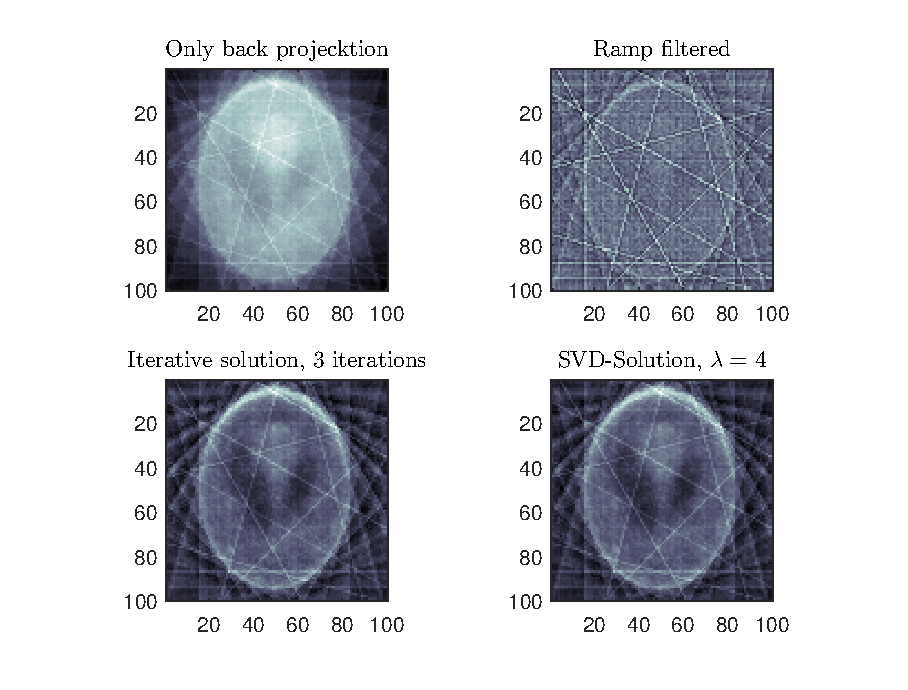
\includegraphics[width=\textwidth]{ALL.eps}
	\caption{Rekonstruktion des Phantombildes $50\times50$ Pixel. Eine Gegenüberstellung aller Verfahren in Bezug auf die Projektionsreduktion. Die Projektionen wurden nur aus 12 Winkel aufgenommen, was insgesamt $p = 1200$ ergibt.}
	\label{fig:3.16}
\end{figure}

In der Abbildung \ref{fig:3.16} ist die Empfindlichkeit der Verfahren gegenüber reduzierter Projektionenanzahl dargestellt. Dieser Aspekt ist in der medizinischen CT- Rekonstruktion von besonderem Interesse. Eine Rekonstruktion mit weniger Projektionen trägt zu einer geringeren Bestrahlungsdosis der Patienten bei. Offensichtlich sind algebraischen Verfahren in dieser Hinsicht die bessere Methoden. Allerdings sind diese für größere Auflösungen im Rekonstruktionsergebnis sehr zeit- und rechenintensiv. Somit sind es die iterativen Verfahren, die sich in der modernen medizinischen CT-Technik immer mehr durchsetzen.

Gegenüber den algebraischen Verfahren ist die gefilterte Rückprojektion sehr schnell und robust. Robust ist sie vor allem deshalb, weil sie alles filtert und zurück projiziert, was im Input reinkommt. Zudem finden dort keine Iterationen statt und es entstehen keine all zu großen Matrizen. Aber, wie die Abbildung (\ref{fig:3.16}) zeigt, ist das Verfahren für kleine Projektionenzahl sehr anfällig. Die gefilterte Rückprojektion wird heutzutage eher in der Materialforschung eingesetzt, weil dort die Strahlenbelastung der untersuchten Objekte keine große Rolle spielt und somit hohe Projektionszahlen erlaubt sind.

Zusammenfassend kann man sagen, dass für die gefilterte Rückprojektion noch mehr Filterkerne implementiert und untersucht werden könnten. Bei der Implementierung des iterativen Verfahrens, könnte noch ein 'klügerer' Fehlerschätzer überlegt werden sowie die Einführung eines Relaxationsparameters, welcher die Konvergenz des Verfahrens steigern könnte. Bei der Rekonstruktion durch SWZ wäre noch zu überlegen, wie die Singulärwerte besser gewichtet werden könnten.